% 这是前沿和背景的一章,主要会介绍对于该问题的研究的意义以及,目前的一些研究状况
\chapter{绪\hspace{1em}论}
\label{cha:intro}
宋代诗人苏东坡说过:“博观而约取,厚积而薄发”。意思是说,只有广见博识才能择其精者而取之。研究如此,研究生生涯亦是如此。研究生生涯作为人生的一部分,从长远来看是一个厚积的过程,这个时期积累的对待问题的态度,见识的众多同行的思想碰撞以及研究过程中的失败与成功等,都会成为今后生活的财富;而短期内,也就是落实到研究中,只有充分调研了问题的背景,了解了国内外了情况并取其精华去其糟粕,准备了充分的数据才能在自己的实际工作中得心应手,做出期望的成果。

绪论作为文章的开始,将为学位论文的展开作铺垫,引领读者进入本文的研究领域——图像集合分类问题。为此,本章首先会在问题的背景和意义进行简要的说明,然后让读者对该问题在国内外的研究现状有个整体把握的同时,对该问题的测试数据和测试协议也有一个大致的了解,最后借助对本文的主体框架的介绍,让读者对文章的结构有一个宏观的把握。
\section{问题的背景与意义}
\label{sec:background}
计算机视觉的任务就是希望给机器赋予等同甚至是超过人类视觉系统对于周围环境的处理能力。图像作为计算机视觉的主要输入,为计算机理解提供丰富信息的同时也给计算机视觉任务带来了挑战:首先,图像是三维空间向二维空间的投影,大量的信息在这个过程中丢失;其次,由于拍摄的角度变化,光照变化以及低分辨率,遮挡等问题使得用单一的图像进行识别、理解等任务变得十分困难;另一方面,由于近年来监控视频,主题相册,用户上传视频,多视角图像数据等都以图像集合的形式呈现出爆发式的增长。图像集合分类问题在这样的大背景下应运而生。

图像集合分类问题的中的数据的主要呈现出两个特点:一是图像的量大,二是图像的质却未必有(大variation)。因而图像集合分类问题的主要任务就是利用量大的特点克服variation大的问题。由于以上的原因,加之数据本身以集合的形式呈现的特点为图像集合分类问题的研究赋予了重要的实践和理论意义。

计算机视觉的任务的大多来源于实际问题的,图像集合的分类也不例外,视频监控就是一个很好的例子,视频监控中的分类识别问题对于警方的网络追逃,海关的出入境管理等的重要性不言而喻;此外,动作识别(动作的描述往往是一段视频输入)对于暴力事件的甄别,预防犯罪也有重要的意义;另一方面,在众多的用户上传的视频数据中不管是做基本的视频检索还是做更深层次的用户行为的分析理解等,图像集合分类问题的研究同样具有重要的意义。

在理论上图像集合分类问题的意义主要体现在:首先,图像数据中的数据是以集合的形式存在,相较于机器学习领域的中的单点(向量)的研究,集合作为输入的研究却不是那么充分;所以图像集合的分类问题的研究对于机器学习中的集合对象的研究有着一定的推动意义;其次,由于数据的独特性,其数学表示也比较特殊,往往是子空间,对称正定矩阵,分布函数,流形等等。而这些非线性结构的表示的研究也将促进机器学习中非线性数据表示的研究。
\section{国内外研究现状}
\label{sec:current}
本节将针对图像集合分类问题在国内外的研究现状进行介绍,帮助读者了解该问题的前沿动态,理解图像集合分类问题本身以及该问题的核心任务和主流的解决方案。
\subsection{符号说明}
\label{sec:symbols}
在进入本节的主要内容之前,由于本文涉及较多数学符号;为了节约篇幅,这里利用表\ref{tab:symbols}统一对本文中的主要符号进行说明。并且本文约定:如无特别说明将使用小写字母(如:$a,b$)表示常量,小写加粗(如:$\bm{x},\bm{y}$)表示向量,大写的字母(如:$X,Y$)表示矩阵,子空间或集合(具体可根据上下文确定),大写字母加粗(如:$\bm{X},\bm{Y}$)表示张量。
\begin{table}[htb]
  \centering
  \begin{minipage}[t]{0.8\linewidth} % 如果想在表格中使用脚注,minipage是个不错的办法
  \caption{符号说明}
  \label{tab:symbols}
    \begin{tabular*}{\linewidth}{lp{10cm}}
      \toprule[1.5pt]
      {\heiti 符号} & {\heiti 说明} \\\midrule[1pt]
      $\mathbb{R}^{n}$ & $n$维向量空间,特别地$\mathbb{R}$表示实数空间 \\
      $M$ & 此符号专用于表示流形(Manifold)\\
      $(S,g)$ &表示黎曼流形(集合$S$以及其上的黎曼度量$g$的二元组),通常为了简单起见也用$S$代替该流形(如:有时也用$\mathbb{S}_{d}^{+}$对称正定矩阵流形),因此$S$的具体意义需要根据上下文确定\\
      $\mathbb{S}_{d}^{+}$ & $d \times d$的对称正定矩阵集合(SPD矩阵)\\
      $\mathbb{S}_{d}^{+}(k)$    & 秩为$k$的$d \times d$半正定矩阵集合(Fixed-Rank PSD矩阵)\\
      $\mathbb{S}_{d}$ & $d \times d$的对称矩阵构成的集合\\
      ${\rm St}(n,k)$   & $n \times k$列满秩矩阵的集合,也表示non-compact Stiefel流形\\
      ${\rm St}^{*}(n,k)$   & $n \times k$列正交矩阵的集合,也表示compact Stiefel流形\\
      ${\rm Gr}(n,k)$   & $\mathbb{R}^{n}$空间中$k$维子空间构成的集合,也表示Grassmann流形\\
      $\log(\cdot)$ & 不做特别说明的话本文中表示的是矩阵的$\log$函数\\
      $\exp(\cdot)$ & 不做特别说明的话本文中表示的是矩阵的$\exp$函数\\
      ${\rm Log}$ & 流形上的${\rm Log}$变换\\
      ${\rm Exp}$ & 流形上的${\rm Exp}$变换\\
      $R$ & 流形上的Retraction变换\\
      ${\rm T}$ & 流形上的Vector Transport变换\\
      $T_{X}M$ & 流形$M$上$X$处的切空间(tangent space)。特别地,$M$上的所有切空间记为$TM$称为$M$上的切空间束\\
      \bottomrule[1.5pt]
    \end{tabular*}
  \end{minipage}
\end{table}
\subsection{图像集合}
\label{sec:Image-Set}
图像集合,顾名思义指的就是多张图片构成的集合,其已经被用于多个领域(视频人脸识别,物体识别,动作识别,表情识别等等),图\ref{fig:image_set_exmples}给出了几个例子。
\begin{figure}[h]
	\subcaptionbox{EXAMP 01: 一段录像\label{fig:subfig_facetrack}(图片来自YTC\cite{Database_YTC}数据库)}
      	{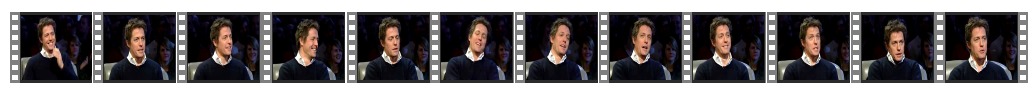
\includegraphics[width=\linewidth]{source/YTC_track.png}}
  	\subcaptionbox{EXAMP 02: 一个物体的Multi-view\label{fig:subfig_apple}(图片来自ETH80\cite{Database_ETH80}数据库)}
      	{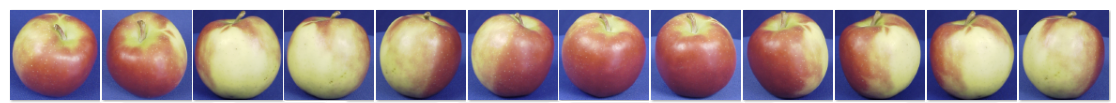
\includegraphics[width=\linewidth]{source/ETH80_apple.png}}
  	\subcaptionbox{EXAMP 03:一个动作描述\label{fig:subfig_motion}(图片来自CMU MoBo\cite{Database_MoBo}数据库)}
    	{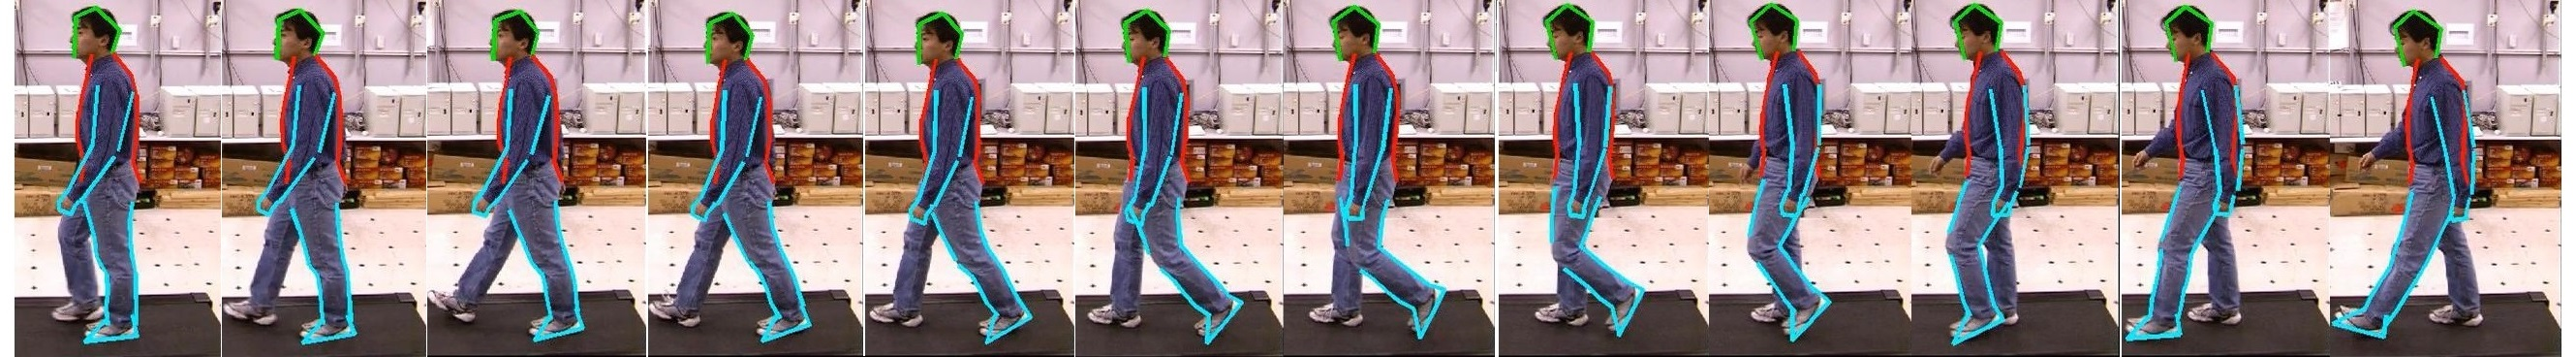
\includegraphics[width=\linewidth]{source/cmu_MoBo.jpg}}
  	\caption{几个图像集合的例子}
  	\label{fig:image_set_exmples}
\end{figure}

图像集合的分类问题的研究和发展已经走过了10多年的时间;在这10多年中,图像集合分类问题从最初被引入CV领域,逐渐成为计算机视觉中的一个研究热点;这个过程中,学者们不断推陈出新,发展出了一系列的方法和路线,为图像集合分类问题的研究做出了重要的探索。

首先,从问题层面可以将图像集合分类问题分为两个大类:图像集合对图像集合的分类问题(Probe和Gallery都是图像集合,在图像集合分类问题中Probe相当于测试集而Gallery相当于训练集),图像集合对静态图像的分类问题(Probe和Gallery中一边是静态图像另一边是图像集合)。其中前者是目前图像集合分类问题研究的主流方向,而后者则是一个新的方向,拥有着广泛的运用前景,在该方向上的一些主要工作有:文献\cite{Statistics_LERM}探究了静态图像到图像集合的分类问题;文献\cite{Statistics_HER}则把静态图像与图像集合的匹配的问题开创性的运用到了视频/图像检索领域;而文献\cite{Affinehull_P2SML}借助Affine Hull表示图像集合,在Metric Learning的框架下,比较全面的讨论了point-to-set以及set-to-set的问题。

图像集合到图像集合的分类问题一直以来是图像集合分类问题的主流的方向,这个问题上按照方法这里进一步的可把图像集合分类问题归纳为如下的几类:1、子空间以及流形建模的方法\cite{Subspace_MSM,Subspace_GDA,Manifold_MMD,Manifold_MDA};2、仿射包建模的方法\cite{Affinehull_AF,Affinehull_SANP,Affinehull_RNP,Affinehull_ProNN};3、统计建模的方法\cite{Statistics_CDL,Statistics_Vemu,Statistics_SPDML,Statistics_LMKML,Statistics_HERML,Statistics_DARG,Statistics_BeyondGauss};4、深度学习的方法\cite{Deeplearning_MMDML,Deeplearning_DRM};5、其它(稀疏编码\cite{Collaborative_ISBCOLREP},协同表示\cite{Dictionary_DBFR}等)。接下来的内容将简要对它们进行介绍。
\subsection{子空间以及流形建模的方法}
\label{sec:current_Subspace_Manifold}
这一类方法出现在图像集合问题研究的早期,为图像集合问题的形成奠定了基础,并且为该问题给出了早期的解决方案。
\subsubsection{子空间建模的方法}
\label{sec:current_SubMan_Subspace}
工作\cite{Subspace_MSM},\cite{Subspace_GDA}是使用子空间建模图像集合的代表,工作\cite{Subspace_MSM}提出了使用图像集合来克服图像大variation的问题(以量取胜),并使用子空间建模图像集合,然后使用主夹角来进行距离度量,工作\cite{Subspace_GDA}进一步的研究了子空间的方法,并且将其统一到Grassmann流形下进行解释。子空间建模图像集合的算法流程可以大致概括如下(参考\cite{Subspace_GDA}):
\begin{itemize}
\item 设$\{\bm{x}_{ij} \in \mathbb{R}^{l}\}_{j=1}^{n_i}$表示第$i$个图像集合,其中$n_i$表示的是集合中的样本数
\item 计算样本均值:$\bar{\bm{x}}_i=\frac{1}{n_i}\sum_{i=1}^{n_i} \bm{x}_{ij}$,样本协方差:$C_i=\frac{1}{n_i-1}\sum_{j=1}^{n_i}(\bm{x}_{ij}-\bar{\bm{x}}_i)(\bm{x}_{ij}-\bar{\bm{x}}_i)^{T}$
\item 对样本协方差做奇异值分解获得:$C_i=U_i\Lambda_iU_{i}^{T}$,指定子空间维数$m(m<l)$,这里假设奇异值分解的结果是按特征值由大到小排序的
\item 获得集合的子空间表示:$Y_i=U_i(:,1:m)$,其中$U_i(:,1:m)$表示取$U_i$的前$m$列
\item 定义两个子空间之间的距离,用于度量$\{Y_j\}_{j=1}^n$的两两之间的距离;在子空间的度量中,主夹角是最主要的概念:
\begin{equation}
\label{principal_angle}
\begin{split}
&\cos \theta_{k}=\max_{\bm{u}_k \in {\rm span(Y_i)}}\max_{\bm{v}_k \in {\rm span(Y_j)}} \bm{u}_{k}^{T}\bm{v}_{k}\\
&~~~~~~~s.t~~\bm{u}_{k}^{T}\bm{u}_{k}=1,\bm{v}_{k}^{T}\bm{v}_{k}=1\\
&\bm{u}_{k}^{T}\bm{u}_{i}=0,\bm{v}_{k}^{T}\bm{v}_{i}=0,(i=1,2,...,k-1)\\
\end{split}
\end{equation}
其物理意义图\ref{fig:principle_angle}所示。
\begin{figure}[h]
	\centering
	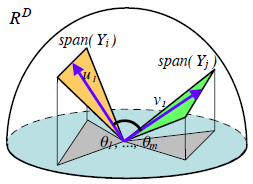
\includegraphics[width=0.4\linewidth]{source/principal_angle.png}
	\caption[子空间之间的主夹角示意图]{子空间之间的主夹角示意图(图片来自文献\cite{Subspace_GDA})}
	\label{fig:principle_angle}
\end{figure}
\item 利用主夹角定义子空间中的距离度量:\\
Projection metric: $d_p (Y_i,Y_j)=\left(∑_{i=1}^m \sin^2 \theta_i\right)^{\frac{1}{2}}$\\
Max correlation: $d_{Max} (Y_i,Y_j)=\left(1-\cos^2\theta_1\right)^\frac{1}{2}$\\
Min correlation: $d_{Min} (Y_i,Y_j)=\left(1-\cos^2\theta_m\right)^\frac{1}{2}$\\
Procrustes metric: $d_{CF} (Y_i,Y_j)=2\left(∑_{i=1}^{m}\sin^2(\theta_i/2)\right)^\frac{1}{2}$
\end{itemize}

工作\cite{Subspace_GDA}进一步在此基础上利用核判别分析(Kernel Discriminant Analysis,KDA)的框架进行了判别学习,在核空间中进行图像集合的分类。
\subsubsection{流形建模的方法}
\label{sec:current_SubMan_Manifold}
流形建模的方法\cite{Manifold_MMD},\cite{Manifold_MDA}假设图像集合中的图像位于流形上(并不充满整个空间),使用多个局部线性空间建模图像集合来估计流形结构,然后利用此结构定义流形与流形之间的距离进行图像集合分类,如图\ref{fig:MMD}所示。
\begin{figure}[h]
	\centering
	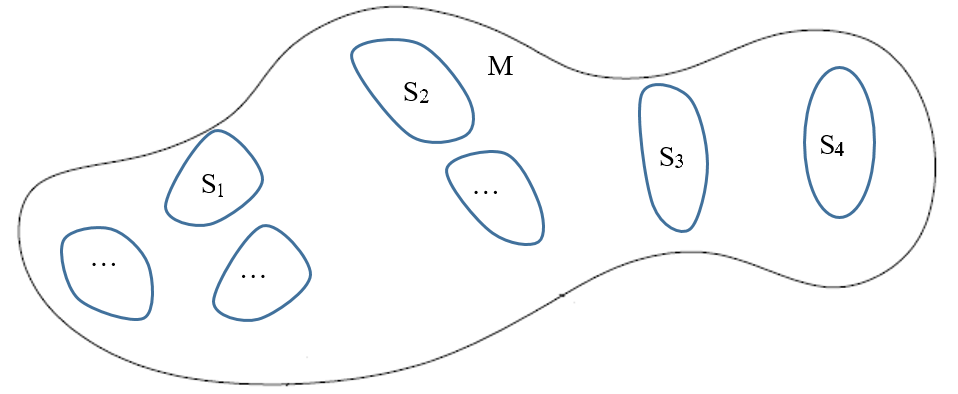
\includegraphics[width=0.7\linewidth]{source/MMD.png}
	\caption{流形的局部线性近似示意图}
	\label{fig:MMD}
\end{figure}
其中$M$表示的是原始的流形结构,文献\cite{Manifold_MMD}根据数据构建局部线性子空间$S_1,S_2,S_3,S_4,...$来近似表示该流形$M$,然后通过点到点的距离定义点到子空间的距离再进一步定义子空间到子空间的距离,最后定义流形到流形的距离,从而进行图像集合的分类(下述定义中的$S,S_{i},C_{j}$表示的的是子空间而不是矩阵)。
\begin{itemize}
\item Point to point distance:$d_{ppd} (\bm{x},\bm{y})=\|\bm{x}-\bm{y}\|$
\item Point to subspace distance: $d_{psd} (\bm{x},S)=\min_{\bm{x}'\in S}\|\bm{x}-\bm{x}'\|$
\item Subspace to subspace distance: $d_{ssd} (S_1,S_2)= any~valid~subspace~metric$
\item Point to manifold distance: $d_{pmd} (\bm{x},M)=\min_{C_i\in M}d_{psd} (\bm{x},C_i )$
\item Subspace to manifold distance: $d_{smd} (S,M)=\min_{C_i\in M}d_{ssd} (S,C_i )$
\item Manifold to manifold distance: $d_{mmd} (M_1,M_2 )=\min_{C_i\in M_1}d_{smd} (C_i,M_2 )$
\end{itemize}
文章\cite{Manifold_MMD}利用上述的Manifold to manifold distance来度量流形之间的距离,然后在此距离上进行图像集合的分类问题,另一篇相关的工作\cite{Manifold_MDA}则是在\cite{Manifold_MMD}的基础上增加了判别信息得到了MDA(Manifold Discriminat Analysis)方法:在构建子空间$S_1,S_2,S_3,S_4,...$的时候要求类内散度尽量小而类间散度尽量大,如图\ref{fig:MDA}所示。
\begin{figure}[h]
	\centering
	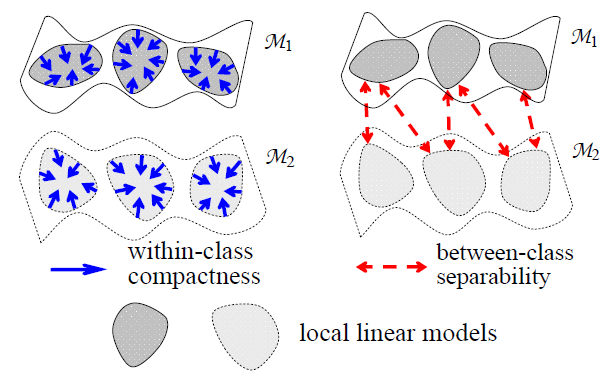
\includegraphics[width=0.7\linewidth]{source/MDA.png}
	\caption[MDA方法示意图]{MDA方法示意图(图片来自\cite{Manifold_MDA})}
	\label{fig:MDA}
\end{figure}
流形建模图像集合的方法是早期的流形学习的概念和图像集合问题的结合,在图像集合分类问题的研究上进行了有益的探索,也为后来的图像集合问题的研究(如\cite{Statistics_DARG,Statistics_BeyondGauss})提供了借鉴意义。
\subsection{仿射包建模的方法}
\label{sec:current_Affinehull}
仿射包建模的方法以其简单有效的特点在图像集合分类问题中被研究者所关注,该方法的代表作有\cite{Affinehull_AF,Affinehull_SANP,Affinehull_RNP,Affinehull_ProNN}。仿射包建模的图像集合的方法最核心的内容就是仿射包(Affine Hull)(由文献\cite{Affinehull_AF}引入到图像集合分类问题中),其定义如公式\ref{affinehull_samples}所示。
\begin{equation}
\label{affinehull_samples}
H_k=\left\{\bm{x}|\bm{x}=\sum_{i=1}^n \alpha_{ki} \bm{x}_{ki},\sum_{i=1}^n \alpha_{ki} =1 \right\}
\end{equation}
其中$k$是图像集合的下标,此外借助空间中的基向量(这里用$U_k$表示基矩阵)的概念还可以定义如下的形式:
\begin{equation}
\label{affinehull_bases}
H_k=\left\{\bm{x}|\bm{x}=\bm{\mu}_k+U_k \bm{v}_k,\bm{v}_k \in \mathbb{R}^l\right\} 
\end{equation}
两个仿射包之间的距离定义如公式\ref{affinehull_dist}所示。
\begin{equation}
\label{affinehull_dist}
D(H_1,H_2)=\min_{\bm{x}\in H_1}\min_{\bm{y}\in H_2}\|\bm{x}-\bm{y}\| 
\end{equation}
如果直接利用公式\ref{affinehull_dist}的定义进行图像集合分类的话容易出现两个仿射包相交(也就是距离为0)的情况,。所以仿射包建模图像集合的一大问题就是对噪声不够鲁棒,针对这个问题\cite{Affinehull_AF}在文献中提出了使用Convex Hull的表示方法(如\ref{affinehull_convex}所示)。
\begin{equation}
\label{affinehull_convex}
H_k^c=\left\{\bm{x}|\bm{x}=\sum_{i=1}^n \alpha_{ki} \bm{x}_{ki},\sum_{i=1}^n \alpha_{ki}=1,L< \alpha_{ki}<U\right\} 
\end{equation}
来建模表示的方案,其中$L,U$分别表示上界和下界(标量),这样做的目的是将$\alpha_{ki}$限制在了一定的范围内来提高了模型对噪声的鲁棒性。

针对Affine Hull对样本不鲁棒的问题,\cite{Affinehull_SANP}提出了使用稀疏表示的方案来解决:
\begin{equation}
\left\{
\begin{split}
\label{affinehull_SANP}
F_{\bm{v}_i,\bm{v}_j}&=\|(\bm{\mu}_i+U_i \bm{v}_i)-(\bm{\mu}_j+U_j \bm{v}_j)\|_{2}^{2}\\
G_{\bm{v}_i,\bm{\alpha}}&=\|(\bm{\mu}_i+U_i \bm{v}_i)-X_i \bm{\alpha}\|_{2}^{2}\\
Q_{\bm{v}_j,\bm{\beta}}&=\|(\bm{\mu}_j+U_j \bm{v}_j)-X_j \bm{\beta}\|_{2}^{2}\\
\min_{\bm{v}_i,\bm{v}_j,\bm{\alpha},\bm{\beta}}&(F_{\bm{v}_i,\bm{v}_j}+\gamma(G_{\bm{v}_i,\alpha}+Q_{\bm{v}_j,\beta})+\lambda_1 \|\bm{\alpha}\|_1+\lambda_2 \|\bm{\beta}\|_1)
\end{split}
\right.
\end{equation}
这样做虽然使得模型对噪声更鲁棒,但是也带来计算复杂度太高的问题;所以\cite{Affinehull_RNP}提出了使用$l_p$范数(通常$p=2$)来代替$l_1$范数。
\begin{equation}
\label{affinehull_RNP}
\min_{\bm{\alpha},\bm{\beta}}\left(\|X\bm{\alpha}-Y\bm{\beta}\|_2^2+\lambda_1 \|\bm{\alpha}\|_{l_p}+\lambda_2 \|\bm{\beta}\|_{l_p}\right),s.t~\sum_{k}\alpha_k =1,\sum_k\beta_k =1
\end{equation}

而文章\cite{Affinehull_ProNN}则使用了高斯模型来增强模型的鲁棒性,使得在最小的误差情况下还要求样本属于该类的概率最大。

最后用图\ref{fig:Affinehull_relation}总结一下仿射包建模图像集合方法之间的关系。
\begin{figure}[h]
	\centering
	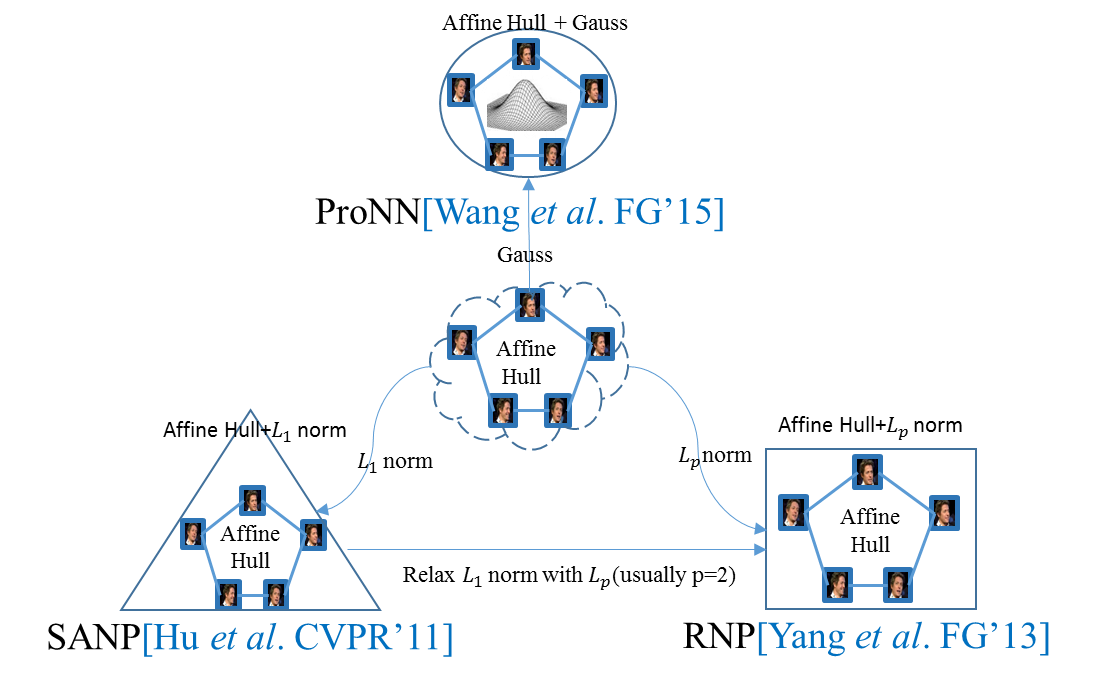
\includegraphics[width=0.7\linewidth]{source/Affinehull_relation.png}
	\caption{仿射包建模图像集合方法关系图}
	\label{fig:Affinehull_relation}
\end{figure}

概括起来就就是:仿射包方法使用仿射包建模图像集合,为了克服直接使用仿射包分类对噪声不鲁棒问题,不同的限制被添加从而衍生出了不同的方法。
\subsection{统计建模图像集合的方法}
\label{sec:current_Statistics}
统计量建模的方法是近年来研究图像集合分类问题的主流方法之一,它以其优越的表现受到越来越多的关注。此外由于统计建模时,数据表示的特殊性(对称正定矩阵(SPD矩阵),分布函数等),黎曼流形成为了主要的研究工具。

统计建模的方法又可以细分为:单一统计量建模的方法,多统模型融合的方法以及基于分布函数的方法:
在单统计量表示图像集合的方法中,协方差矩阵被认为是丰富而有效的特征表示,样本协方差矩阵:$C=\frac{1}{n-1}\sum_{i=1}^n (\bm{x}_i-\bar{\bm{x}})$,其中$\bar{\bm{x}}=\frac{1}{n}\sum_{i=1}^n \bm{x}_i$为样本均值(协方差矩阵一般是正定的$C \succ 0$,因此其并不构成欧氏空间),图\ref{fig:2d_SPD_cone}给出了2*2对称正定矩阵在三维空间中的例子\footnote{需要注意的是:$2\times 2$对称正定矩阵组成的集合本身并不包含这些外边界(因为它是开集),而是该边界包住的整个锥的内部}。
\begin{figure}[h]
	\centering
	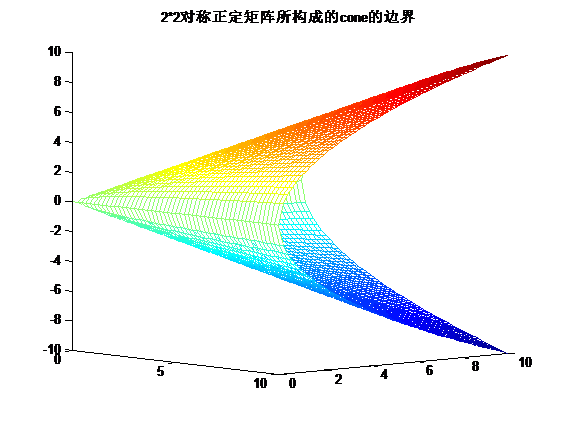
\includegraphics[width=0.5\linewidth]{source/2d_SPD_cone.png}
	\caption{$2\times 2$对称正定矩阵的外边界在3维空间中的结构}
	\label{fig:2d_SPD_cone}
\end{figure}

协方差建模图像集合的代表作\cite{Statistics_CDL}:利用核函数$\phi=\log(.)$将协方差矩阵流形映射到RKHS空间,在新的RKHS空间中,使用KPLS\cite{Kernel_KPLS}回归以及KDA\cite{Kernel_KDA}对视频人脸,多视角图像集等图像集合数据进行分类。

文献\cite{Statistics_SPDML}则在对称正定矩阵(SPD)集合中,利用黎曼度量进行协方差降维及判别学习,算法的优化的空间(投影矩阵所在的空间)为Grassmann流形。

多统计模型融合的方法主要的代表作有\cite{Statistics_LMKML}和\cite{Statistics_HERML},两者的思想比较近似,主要思想是:不同的统计模型会刻画目标的不同侧面,包含了不同的信息,融合它们可以得到目标的更全面的表示。在具体实现过程中,工作\cite{Statistics_LMKML}首先利用核映射将不同统计模型映射到再生核希尔伯特空间(Reproducing Kernel Hilbert Space,RKHS)中,然后利用局部多核度量学习将其整合到一起进行分类,其算法流程如图\ref{fig:subfig_LMKML}所示。工作\cite{Statistics_HERML}首先也利用核函数将不同的统计模型映射到统一的再生核希尔伯特空间空间中,然后在新的再生核希尔伯特空间中利用融合的特征进行分类,其核心内容可以用图\ref{fig:Multi_Stat}描述。
\begin{figure}[h]
  \centering
  \subcaptionbox{LMKML\cite{Statistics_LMKML}方法流程图\label{fig:subfig_LMKML}(图片来自\cite{Statistics_LMKML})}
      {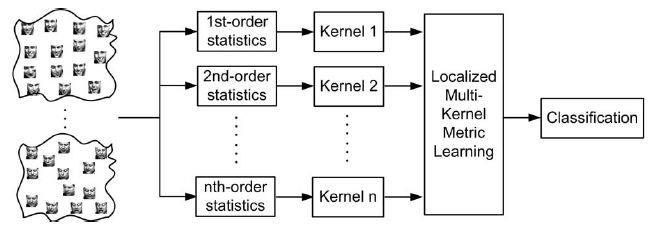
\includegraphics[width=0.51\linewidth]{source/Statistics_LMKML.png}}
  \hspace{1em}%
  \subcaptionbox{HERML\cite{Statistics_HERML}方法流程图\label{fig:subfig_HERML}(图片来自\cite{Statistics_HERML})}
      {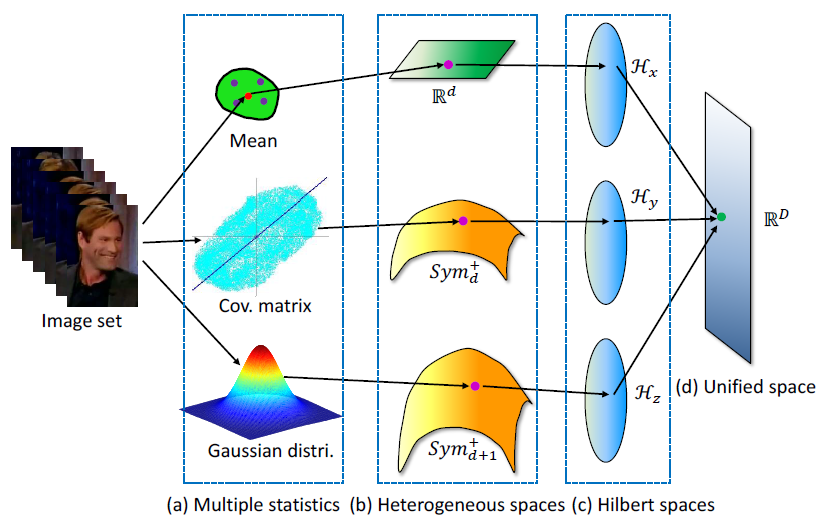
\includegraphics[width=0.45\linewidth]{source/Statistics_HERML.png}}
  \caption{多统计模型建模图像集合方法}
  \label{fig:Multi_Stat}
\end{figure}

为了更好的挖掘图像集合原始分布的信,分布函数建模图像集合的方法被提出:文献\cite{Statistics_DARG}使用高斯混合模型(GMM)表示图像集合(逼近原始分布),利用核映射将GMM的各个component映射到RKHS中,并在核判别学习(Kernel Discriminant Analysis,KDA)\cite{Kernel_KDA}的框架下学习投影矩阵,最后在投影空间中分类;而文献\cite{Statistics_BeyondGauss}则使用KDE(Kernel Density Estimation)表示图像集合(逼近原始分布),并设计距离/散度来度量两个图像集合的KDE表示的距离,为了使得KDE估计可靠,文章中还为数据学习一个具有判别性的降维矩阵$W$来辅助估计。

统计建模图像集合的方法小结:1)统计建模的方法从最初的单统计量模型开始,经过发展逐步形成多统计模型融合以及分布函数建模图像集合等一系列方法;2) 由于数据表示的特殊性,统计模型的数学表示往往与黎曼流形相关联,黎曼流形成了研究它们的一个重要工具。图\ref{fig:Statistics_relation}描述了已有的统计建模图像集合的方法的一些关系。
\begin{figure}[h]
	\centering
	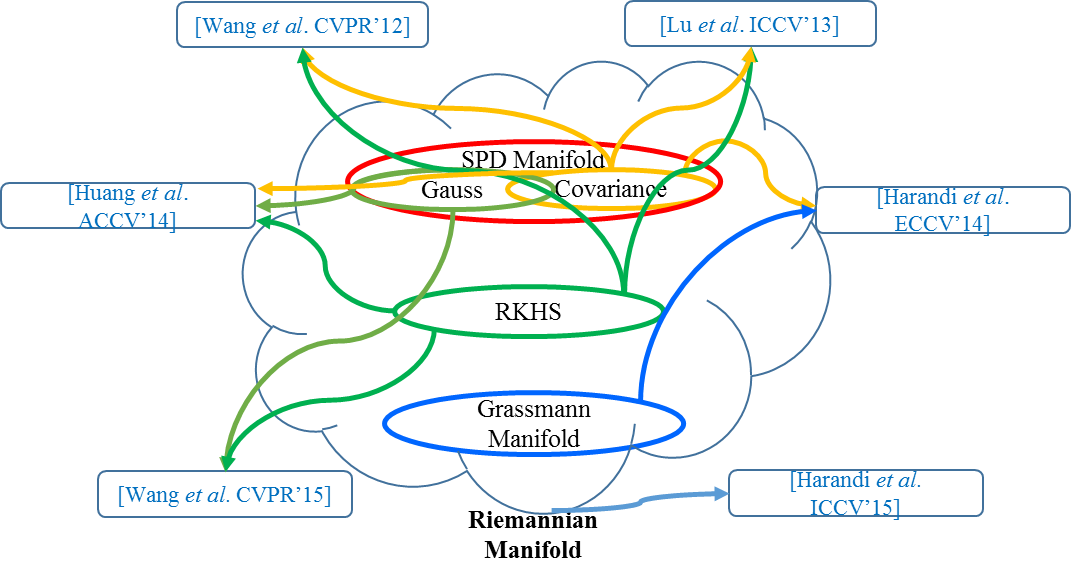
\includegraphics[width=0.7\linewidth]{source/Statistics_relation.png}
	\caption{统计建模图像集合的方法间的关系}
	\label{fig:Statistics_relation}
\end{figure}
\subsection{深度学习的方法}
\label{sec:current_Deeplearning}
深度学习在众多的领域都取得了不小的成果,所以也有学者将深度学习(Deep Learning,DL)的方法用于图像集合分类.目前这种尝试的主流做法是为每类学一个网络,并期望深度网络能够学到原始流形的geometry的结构。两个代表性的工作是:文献\cite{Deeplearning_DRM}为每类学一个AE-Like(Unsupervised)网络(网络结构如图\ref{fig:subfig_DRM}所示),自动挖掘Manifold的Geometry结构,最终利用重建误差以及voting进行分类。
\begin{figure}[h]
  \centering
  \subcaptionbox{DRMs-WV\cite{Deeplearning_DRM}方法网络结构\label{fig:subfig_DRM}(图片来源于\cite{Deeplearning_DRM})}
      {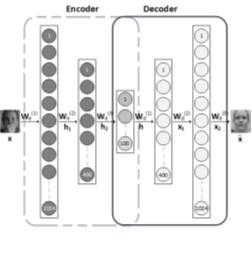
\includegraphics[width=0.3\linewidth]{source/Deeplearning_DRM.png}}
  \hspace{4em}%
  \subcaptionbox{MMDML\cite{Deeplearning_MMDML}方法流程图\label{fig:subfig_MMDML}(图片来自\cite{Deeplearning_MMDML})}
      {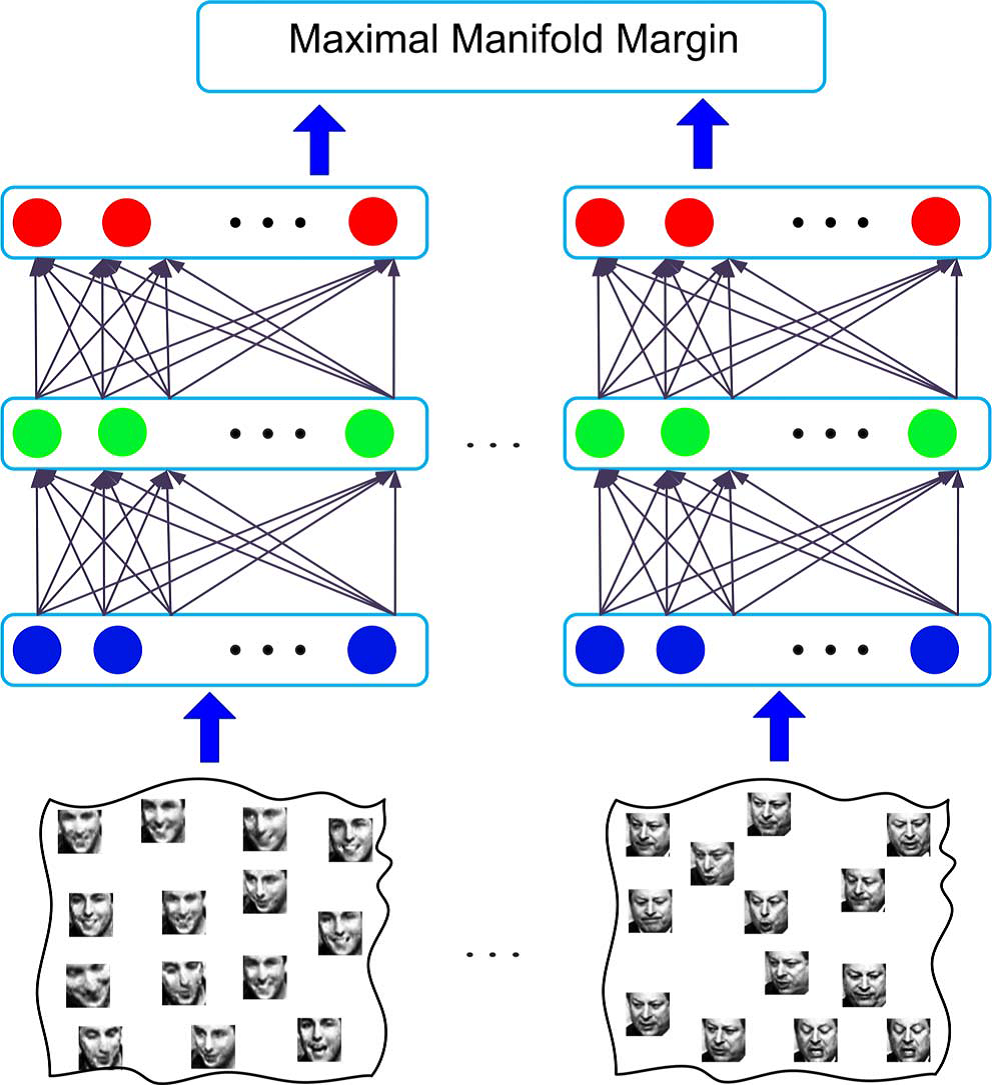
\includegraphics[width=0.3\linewidth]{source/Deeplearning_MMDML.png}}
  \caption{深度学习建模图像集合的代表性网络结构}
  \label{fig:Deepleaning_Nets}
\end{figure}

文献\cite{Deeplearning_MMDML}为每类学一个DNN-Like(Supervised)网络,使得在输出层不同类的margin尽量大;其网络结构如图\ref{fig:subfig_MMDML}所示。

深度学习将计算机视觉的发展推向了一个新的高度,也为图像集合的研究注入了新的活力,所以这里使用一定的篇幅对其进行系统的介绍;由于工作\cite{Deeplearning_MMDML}是对工作\cite{Deeplearning_DRM}的改进,所以这里仅以MMDML\cite{Deeplearning_MMDML}为例对该类方法做一个介绍:在L+1层的DNN网络中,对于第$c$个图像集合的第$i$张图片其顶层输出如公式\ref{L_layer_output}所示。
\begin{equation}
\label{L_layer_output}
\bm{h}_{ci}^{L}=s(W_{c}^{L}\bm{h}_{ci}^{L-1}+\bm{b}_{c}^{L})
\end{equation}
其中$W_c^L$是投影矩阵,$\bm{b}_c^L$是偏置向量,$\bm{h}_{ci}^{L-1}$是上一层输出,$s(.)$为非线性激活函数;MMDML\cite{Deeplearning_MMDML}方法在网络顶层最大化不同manifold之间的margin;为此,工作\cite{Deeplearning_MMDML}为每类的每个样本(如第$c$类的第$i$个样本)定义公式\ref{MMDML_neighbor_descri}中的近邻关系描述。
\begin{equation}
\label{MMDML_neighbor_descri}
\left\{
\begin{split}
&D_1 (\bm{h}_{ci}^L )=\frac{1}{K_1}\sum_{p=1}^{K_1}\|\bm{h}_{ci}^{L}-\bm{h}_{cip}^L\|_2^2\\
&D_2 (\bm{h}_{ci}^L )=\frac{1}{K_1}\sum_{q=1}^(K_2)\|\bm{h}_{ci}^L-\bm{h}_{ciq}^L\|_2^2 
\end{split}
\right.
\end{equation}
其中$\bm{h}_{cip}^L$表示的是当前样本的第$p$个同类近邻在网络顶层的输出,$\bm{h}_{ciq}^L$表示的是当前样本的第$q$个不同类的近邻在网络顶层的输出,$K_1,K_2$是两个设置近邻个数的参数。故上式定义了第$c$类的第$i$个样本在网络顶层与$K_1$个同类近邻,$K_2$个不同类近邻的关系。

MMDML方法的目标是在网络顶层最大化不同manifold之间的margin:

首先使用$f_c=[W_c^1,W_c^2,\cdots,W_c^L,\bm{b}_c^1,\bm{b}_c^2,\cdots,\bm{b}_c^L]$表示网络参数,然后定义:
\begin{equation}
\label{Layer_Loss}
\left\{
\begin{split}
&H_1=\sum_{c=1}^C\sum_{i=1}^{N_c}g(D_1(\bm{h}_{ci}^{L})-D_2(\bm{h}_{ci}^L))\\
&H_2=\sum_{c=1}^C\sum_{l=1}^L(\|W_{c}^{l}\|_{F}^{2}+\|\bm{b}_{c}^{l}\|_{2}^2)
\end{split}
\right.
\end{equation}

其中$N_c$表示第$c$个图像集合中的样本数。利用公式\ref{Layer_Loss}得到MMDL的优化目标:
\begin{displaymath}
\min_{f_1,f_2,\cdots,f_C }H= H_1+\frac{1}{2}H_2
\end{displaymath}

文献\cite{Deeplearning_MMDML}中使用了随机次梯度下降算法训练网络参数,在最后在测试阶段,测试样本的分类结果由公式\ref{MMDML_classify}获得。
\begin{equation}
\label{MMDML_classify}
L_q=\arg\min_c d(X_q,X_c),1\leq c\leq C
\end{equation}
其中$X_q=[\bm{x}_1^q,\bm{x}_2^q,\cdots,\bm{x}_{N_q}^q]$表示的是测试数据$X_c$表示的是训练数据,而$d(X_q,X_c)$的计算过程如下:1)使用网络将$\bm{x}_j^q$映射到新的空间$\bm{h}_c (\bm{x}_j^q )$;2)计算$\bm{h}_c (\bm{x}_j^q )$与$\bm{h}_{ci}^L,i=1,2,\cdots,N_c$的欧氏距离,并将最小的距离作为$\bm{x}_j^q$与第$c$个manifold的距离,最后对所有样本$\bm{x}_1^q,\bm{x}_2^q,\cdots,\bm{x}_{N_q}^q$求平均作为$d(X_q,X_c)$。
\subsection{国内外研究现状小结}
\label{sec:current_Summarize}
总结国内外对图像集合分类问题的研究,对图像集合分类问题的研究可做如下描述:1)为图像集合设计一种表示(子空间、流形、仿射包、统计模型及深度网络等);2)为这种表示(模型)设计/定义一种距离度量,并用距离/度量进行判别学习;3)(可选)针对已有模型问题(不鲁棒、维度太高……)做进一步改进。

另一方面,在图像集合分类问题中,由于数据的特殊性,往往需要对非线性的数据进行研究,在子空间、统计建模等方法中,黎曼流形作为成熟的数学工具在其中发挥了重要的作用。 

最后,还需要注意到除了前面介绍的一些方法,还有其它一些方法,如:稀疏编码和协同表示的方法也为图像集合的分类问题的探索做出了重要贡献。
\section{数据介绍}
\label{sec:data_intro}
图像集合分类问题来源于实际问题,最终还是要回到实际问题中;所以只有理论还是不够,还需要数据的支撑;本小节就是对图像集合分类问题中的一些常用的数据集进行介绍;此外,多样化的数据也更能说明算法的有效性,并且由于本文对黎曼流形问题的研究过程中并没有限制在图像集合问题上,所以这里还会介绍一个可用黎曼流形建模的数据集合,表格\ref{tab:database_list}中列出了本节将要介绍的数据库。
\begin{table}[htb]
	\centering
	\caption{数据库列表}
	\begin{tabular}{l|l|c}
	\toprule[1.5pt]
		{\heiti 数据库} &{\heiti 描述} &{\heiti 备注} \\ \hline
		YouTube Faces DB\cite{Database_YTF} &1595个人,3425段视频,低分辨高压缩率 &人脸数据库 \\ \hline
		YouTube Celebrity\cite{Database_YTC} &47个人,1910段视频, 低分辨高压缩率 &人脸数据库 \\ \hline
		UIUC\cite{Database_UIUC} &4个大类,18个子类,每类12张图片 &材料(material)数据库 \\ \hline
		ETH-80\cite{Database_ETH80}   &共8个子类每类4个图像集合每个集合41张图片 &物体识别数据库 \\ \hline
		CMU MoBo\cite{Database_MoBo} &25个人,4个运动(行走)类,150段视频数据 &为步态研究而搜集 \\
	\bottomrule[1.5pt]
	\end{tabular}
	\label{tab:database_list}
\end{table}\\
图\ref{fig:databases_exmples}给出这些数据集的一些示例图片。
\begin{figure}[htb]
	\centering
	\subcaptionbox{YouTube Faces DB\cite{Database_YTF}数据库示例\label{fig:subfig_database_YTF}}
      	{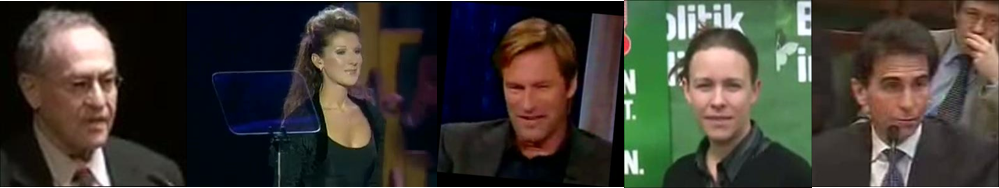
\includegraphics[width=0.49\linewidth]{source/YTF.png}}
  	\subcaptionbox{YouTube Celebrity\cite{Database_YTC}数据库实例\label{fig:subfig_database_YTC}}
      	{
\includegraphics[width=0.49\linewidth]{source/YTC.png}}
  	\subcaptionbox{UIUC\cite{Database_UIUC}数据库示例\label{fig:subfig_database_UIUC}}
    	{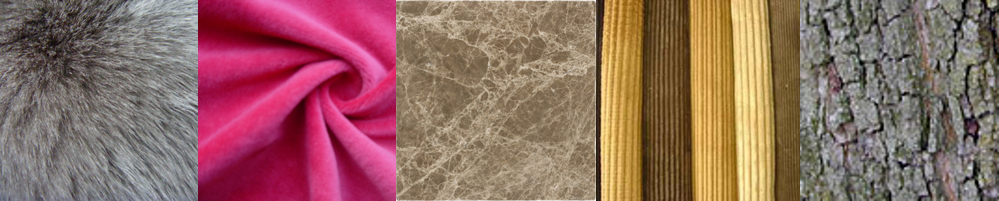
\includegraphics[width=0.49\linewidth]{source/UIUC.png}}
    \subcaptionbox{ETH80\cite{Database_ETH80}数据库示例\label{fig:subfig_database_ETH80}}
      	{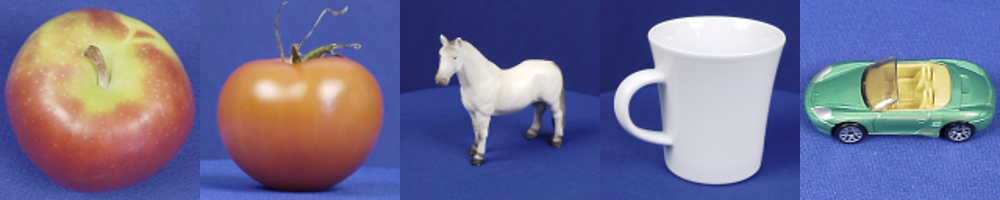
\includegraphics[width=0.49\linewidth]{source/ETH80.png}}
    \subcaptionbox{CMU MoBo\cite{Database_MoBo}数据库示例\label{fig:subfig_database_CMU_MoBo}}
      	{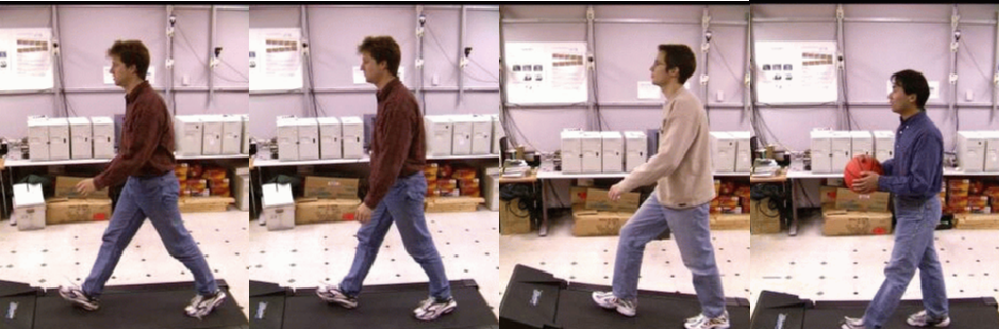
\includegraphics[width=0.5\linewidth]{source/CMUMoBo.png}}
  	\caption{数据库示例}
  	\label{fig:databases_exmples}
\end{figure}
YouTube Faces DB数据库\cite{Database_YTF}最初是为视频人脸验证任务收集的,其收集过程中根据LFW(Labeled Faces in the Wild)\cite{Database_LFW}数据集的样本进行,数据库包含了1595个人的3425个视频段,是一个较大的视频数据库,这些数据均从Youtube上获得,最短的只有48帧,最长的则有6070帧;由于数据是从网络中收集的所以存在脸部姿态变化,表情变化等一系列问题。

Youtube Celebrity数据集\cite{Database_YTC}也是从YouTube上收集而来,最初是为人脸跟踪和识别任务而收集的,数据集包含47个人的1910个视频段,属于是较大的一个视频数据库。其数据呈现出低分辨率和高压缩率的特点,此外同样存在脸部姿态变化、表情变化等问题。数据库的状况比较接近于真实情况,识别任务有不小的挑战。

UIUC数据库\cite{Database_UIUC}是材料数据库(material database),数据库的组织结构大致为:顶层是四个大类,分别是树皮、织物、建筑材料和动物的皮毛,下面分出18个子类,每个子类包含了12张图像,该数据集并不属于图像集合的数据集,但是当使用Region Covariance为图像建模表示的时候,该数据集上的分类问题研究也将与SPD矩阵黎曼流形相关。

ETH80数据库\cite{Database_ETH80}主要用于物体识别任务,数据集中的数据从概念上属于4个大类:水果蔬菜类、动物类、(小型的)人造的类别及(大型的)人造的类别,具体采集了8个类别:苹果、牛、杯子、狗、马、梨、西红柿、和汽车,整个数据集包含80个图像集合(每个类别10个集合),每个集合包含41张图片,所以数据集总大小为3280张图片。

CMU MoBo数据库\cite{Database_MoBo}包含25个人在室内环境下,跑步机上的6个view行走姿态的150段视频数据,数据库中的数据主要有4种行走姿态(摄像机帧率30FPS):慢速行走,快速行走,斜面行走以及带球行走。

在本节的最后简单的介绍一下测试协议的问题,其中由于CMU MoBo\cite{Database_MoBo}提出的时间相对比较早,所以这里不再介绍它的测试协议,此外该数据集也不会在实际的实验中使用。而YouTube Faces DB数据库由于做的是人脸验证任务,与分类识别任务有所区别,在本文的实际实验中也没有列入,但是考虑到今后可能会用到这个数据库(毕竟它是相当大的视频人脸数据库)所以这里仍然简单介绍一下它的测试协议。在所有的数据集上均采用了10折交叉验证,最后报告的结果均是10则交叉验证的平均结果,其中在每一次验证过程中我们将训练集称为Gallery测试集称为Probe,在各个数据集合上对数的划分情况如下:在YTF(YouTube Faces DB)上根据文献\cite{Database_YTF}中的方式,将数据库提供的5000对视频对平均分为10份(每份500对,其中250对的每对是同一个人,另外250对的每对不是同一个人)。在YTC(YouTube Celebrity)\cite{Database_YTC}上数据的划分则是参考了\cite{Statistics_CDL}以及\cite{Statistics_Vemu}的数据划分方式,在YTC数据集合上对每个人随机选取3个视频段作为训练(Gallery)6个视频段作为测试(Probe),然后将这个过程重复进行10次来获得数据集的随机划分。在UIUC数据库\cite{Database_UIUC}上的数据划分比较简单,我们随机从每个子类中选取一半的样本做为训练集(Gallery)剩下的一半的数据作为测试集(Probe),然后也重复这个过程10次得到10次验证的数据。ETH80数据上的数据划分也参考了\cite{Statistics_CDL},其上的数据划分是在每个类别中随机选取5个图像集合作为训练集(Gallery)剩下的5个作为测试集(Probe),并重复这个过程10次作为10次验证的数据。以上便是本文中使用的数据库的数据划分方式和测试协议。
\section{本文的组织结构}
\label{sec:struct}
在本章的最后,我们来介绍一下本文的组织结构:第一章是绪论,这一章主要介绍问题的背景意义以及国内外的研究现状。作为本文的第一章主要目的是引领读者对图像集合分类问题有一个宏观的了解,也为后续自己工作的介绍做准备。

第二章将介绍矩阵函数与黎曼流形上的优化问题,这部分的内容通过对黎曼流形,矩阵函数等基本概念的介绍,对矩阵函数求导和流形优化等一般化的问题进行了初步的探究。并结合本文其它两个研究内容中的一些实际问题对其进行展开,目的是方便读者理解和实现本文中的提到的方法和概念的同时,帮助读者在遇到类似问题的时候能够从中获得启示。

第三章介绍黎曼流形上的偏最小二乘问题,这一章的内容会从欧氏空间的偏最小二乘问题开始介绍,然后借助投影的一般形式将其扩展到黎曼流形中得到黎曼流形上偏最小二乘问题的基础版本的,紧接着是结合流形的特点以及考虑到数据的稀疏性问题,从基础版本的黎曼流形上的偏最小二乘问题出发提出了多切空间逐步回归的偏最小二乘学习方法,最后实验验证了该方法。

第三章简单回顾了使用子空间和协方差矩阵表示图像集合的方法的问题后,考虑使用半正定(PSD)矩阵表示图像集合,在对早期工作以及工作\cite{PSD_WACV}中的不足进行分析之后,提出了使用嵌入判别信息的Low-Rank PSD矩阵建模图像集合的方法,最终实验验证了该建模方法的有效性。

第五章总结和讨论前几章的内容,对现有研究做了回顾与不足之处的分析,并对下一步可能的方向做了讨论和展望。